\documentclass[10pt,journal,cspaper,compsoc]{IEEEtran}
%
% If IEEEtran.cls has not been installed into the LaTeX system files,
% manually specify the path to it like:
% \documentclass[12pt,journal,compsoc]{../sty/IEEEtran}

\usepackage{fixltx2e}
% \usepackage{stfloats}
\usepackage{amsmath}
\usepackage{graphicx}
\usepackage{amsfonts}
\usepackage{amsthm}
\usepackage{cite}
\usepackage{algorithm}
\usepackage{algorithmic}
\usepackage{url}
\input{/Users/jovo/Research/latex/latex_commands.tex}
\hyphenation{op-tical net-works semi-conduc-tor}
\newcommand{\Qs}{Q}
% \newcommand{\mcL}{\mc{L}}
\newcommand{\mcS}{\mc{S}}
\newcommand{\mcU}{\mc{U}}


\begin{document}

\title{Bayes Optimal Graph Classification: Applications in Statistical Connectomics}

\author{Joshua T.~Vogelstein %, Mark Dredze, R.~Jacob~Vogelstein, 
 and 
Carey~E.~Priebe% <-this % stops a space
\IEEEcompsocitemizethanks{\IEEEcompsocthanksitem J.T. Vogelstein and C.E. Priebe are with the Department
of Applied Mathematics and Statistics, Johns Hopkins University, Baltimore, MD 21218.  %\protect\\
% note need leading \protect in front of \\ to get a newline within \thanks as
% \\ is fragile and will error, could use \hfil\break instead.
E-mail: \{joshuav,cep\}@jhu.edu
% \IEEEcompsocthanksitem R.J. Vogelstein is with the Johns Hopkins University Applied Physics Laboratory, Laurel, MD, 20723.
}% <-this % stops a space
\thanks{}}
 
% The paper headers
\markboth{IN PREP}%
{Graph Classification}

\IEEEcompsoctitleabstractindextext{%
\begin{abstract}
Graph classification algorithms often do not incorporate vertex label information in their classifiers.  In this work, we investigate the extent to which discarding vertex labels can hinder classification performance, and for which random graph models it would be expected to matter.  Via theory we demonstrate a collection of results.  Specifically, if one ``shuffles'' the graphs prior to classification, the vertex label information is irretrievably lost, which can degrade misclassification performance (and does whenever the vertex labels have class-conditional signal).  Thus, while one cannot hope to recover the labels, trying to recover the labels actually results in a consistent estimate of the optimal graph invariant.  This approach therefore solves the question of ``which invariant to use'' for any graph classification problem, at least asymptotically.  Via simulation we demonstrate that a finite (and small) number of training samples can be sufficient to achieve this bound.  Finally, we apply this approach to a ``connectome'' classification problem (a connectome is the complete set of connections within a brain).  Unshuffling the graphs indeed improves performance, although not over the best performance achievable composing a number of graph invariant and machine learning tools.  Thus, given any unlabeled graph classification problem, the relative performance of an unshuffling approach might be difficult to predict with small sample sizes.
\end{abstract}

% Note that keywords are not normally used for peer review papers.
\begin{keywords}
statistical inference, graph theory, network theory, structural pattern recognition, connectome.
\end{keywords}}


% make the title area
\maketitle
\IEEEdisplaynotcompsoctitleabstractindextext
\IEEEpeerreviewmaketitle



\section{Introduction} \label{sec:1}

\IEEEPARstart{T}{his} work addresses graph classification in the presence of vertex label shuffling.   
% Consider the following idealized scenario. 
A (labeled) graph $G=(\mc{V},\mc{E})$ consists of a vertex set, $\mc{V}=[n]$, where $n < \infty$ is the number of vertices and $[n]=\{1,\ldots, n\}$, and an edge set $\mc{E} \subseteq \binom{[n]}{2}$.  Vertex labels may or may not be observed.  In the latter case, vertex $v$ in one graph cannot be assumed to correspond to vertex $v$ in another graph.

MOTIVATION


% Graph classification differs from classification of vector-valued random variables in several key aspects.  First, the structure of a graph may encode information.  Second, the vertex labels may or may not be observed.  In unobserved scenarios, NP-hard problems rear their ugly heads \cite{Conte2004}. 


\section{Graph Classification Models} % (fold)
\label{sec:shuffler_graph_class_models}

\subsection{A labeled graph classification model} % (fold)
\label{sub:a_labeled_graph_classification_model}

% subsection a_labeled_graph_classification_model (end)

 Let $\GG\colon \Omega \to \mc{G}_n$ be a graph-valued random variable taking values $G\in \mc{G}_n$, where $\mc{G}_n$ is the set of graphs on $n$ vertices, and $|\mc{G}_n|=2^{\binom{n}{2}}=d_n$. 
Let $Y$ be a categorical random variable, $Y\colon \Omega \to \mc{Y}=\{y_1,\ldots, y_{c}\}$, where $c< \infty$.  Assume the existence of a joint distribution, $\PP_{\GG,Y}$ which can be decomposed into the product of a class-conditional distribution (likelihood) $\PP_{\GG|Y}$ and a class prior $\pi_Y$. Because $n$ is finite, the class-conditional  distributions $\PP_{\GG | Y=y}=\PP_{\GG|y}$ can be considered discrete distributions $\text{Discrete}(G; \bth_y)$, where $\bth_y$ is an element of the $d_n$-dimensional unit simplex $\triangle_{d_n}$ (satisfying $\theta_{G|y}\geq 0$ $\forall G \in \mc{G}_n$ and $\sum_{G \in \mc{G}_n} \theta_{G|y}=1$).


% $\bth_y=[\theta_{1|y},\ldots \theta_{d|y}]\T \in \triangle_d$, where  $d=|\mc{G}_n|=2^{\binom{n}{2}}$ and $\triangle_d$ is the $d$-dimensional simplex (that is, $\theta_{i|y}\geq 0$ for all $i \in [d]$ and $\sum_{i \in [d]} \theta_{i|y}=1$). 

\subsection{A shuffled graph classification model} % (fold)
\label{sub:a_shuffled_graph_classification_model}

% subsection a_shuffled_graph_classification_model (end)

In the above, it was implicitly assumed that the vertex labels were observed.  However, in certain situations (such as the motivating connectomics example presented in Section \ref{sec:1}), this assumption is unwarranted.  To proceed, we define two graphs $G,G' \in \mc{G}_n$ to be isomorphic if and only if there exists a vertex permutation (shuffle) function $\Qs\colon\mc{G}_n \to \mc{G}_n$ such that $\Qs(G)=G'$.  Let $\QQ$ be a permutation-valued random variable, $\QQ\colon\Omega \to \mc{Q}_n$, where $\mc{Q}_n$ is the space of vertex permutation functions on $n$ vertices so that $|\mc{Q}_n|=n!$.  Extending the model to include this vertex shuffling distribution yields $\PP_{\QQ,\GG,Y}$.  We assume throughout this work (with loss of generality) that the shuffling distribution is both \emph{class independent} and \emph{graph independent}; therefore, this joint model can be decomposed as
\begin{align}
	\PP_{\QQ,\GG,Y} = \PP_{\QQ} \PP_{\GG,Y} = \PP_{\QQ} \PP_{\GG |Y} \pi_Y.
\end{align}
As in the labeled case, the shuffled graph class-conditional distributions $\PP_{\QQ(\GG)|y}$ can be represented by discrete distributions $\text{Discrete}(G; \bth_y')$, where again $\bth_y' \in \triangle_{d_n}$.  When $\PP_{\QQ}$ is uniform on $\mc{Q}_n$, all shuffled graphs within the same isomorphism set are equally likely; that is  $\{\theta_{G_i|y}' = \theta_{G_j|y}' \, \forall G_i,G_j \colon \Qs(G_i)=G_j$ for some $\Qs \in \mc{Q}_n\}$.


\subsection{An unlabeled graph classification model} % (fold)
\label{sub:an_unlabeled_graph_classification_model}

% subsection an_unlabeled_graph_classification_model (end)

Let $\mt{\mc{G}}_n$ be the collection of isomorphism sets.
An \emph{unlabeled graph} $\mt{G}$ is an element of $\mt{\mc{G}}_n$. The number of unlabeled graphs on $n$ vertices is $|\mt{\mc{G}}_n|=\mt{d}_n \approx d/n!$ (see \cite{A000088} and references therein).
% , and $|\mt{\mc{G}}_n|=\mt{d}_n$.  
An \emph{isomorphism function} $U\colon \mc{G}_n \to \mt{\mc{G}}_n$ is a function that takes as input a graph and outputs the corresponding unlabeled graph. Let $\mt{\GG}\colon \Omega \to \mt{\mc{G}}_n$ be an unlabeled graph-valued random variable taking values $\mt{G} \in \mt{\mc{G}}_n$.   The joint distribution over unlabeled graphs and classes is therefore
$\PP_{\mt{\GG},Y}=\PP_{U(\GG),Y}=\PP_{U(\QQ(\GG)),Y}$, which decomposes as $\PP_{\mt{\GG}|Y} \pi_Y$. The class-conditional distributions $\PP_{\mt{\GG} | y}$ over isomorphism sets (unlabeled graphs) can also be thought of as discrete distributions $\text{Discrete}(\mt{G}; \mb{\mt{\theta}}_y)$ where $\mb{\mt{\theta}}_y\in \triangle_{\mt{d}_n}$ are vectors in the $\mt{d}_n$-dimensional unit simplex.   Comparing shuffling and unlabeling for the independent and uniform shuffle distribution $\PP_{\QQ}$, we have $\{\theta_{G|y}'=\mt{\theta}_{\mt{G}|y}/|\mt{G}|$ for all $G \in \mt{G}\}$.  




\section{Bayes Optimal Graph Classifiers} % (fold)
\label{sec:bayes_optimal_graph_classifiers}

We consider graph classification in the three scenarios described above: labeled, shuffled, and unlabeled.  To proceed, in each scenario we define three mathematical objects: (i) a classifier, (ii) the Bayes optimal classifier, and (iii) the Bayes risk.

\subsection{Bayes Optimal Labeled Graph Classifiers} % (fold)
\label{sub:labeled_graph_classifiers}

% subsection labeled_graph_classifiers (end)

% \begin{itemize}
	% \item 
	A \emph{labeled graph classifier} $h\colon \mc{G}_n \to \mc{Y}$ is any function that maps from labeled graph space to class space. The risk of a labeled graph classifier under $0-1$ loss is the expected misclassification rate $L(h)=\EE[h(\GG)\neq Y]$, where the expectation is taken against $\PP_{\GG,Y}$.
	% \item  
	
	The \emph{labeled graph Bayes optimal classifier} is given by
	\begin{align}
		h_* = \argmin_{h \in \mc{H}} L(h),
	\end{align}
	where $\mc{H}$ is the set of possible labeled graph classifiers.
	% \item 
	
	The \emph{labeled graph Bayes risk} is given by 
	\begin{align}
		L_* =\min_{h \in \mc{H}} L(h),
	\end{align}
	where $L_*$ implicitly depends on $\PP_{\GG,Y}$.
% \end{itemize}



% A \emph{labeled} graph classifier $h\colon \mc{G}_n \to \mc{Y}$ is any function that maps from graph space to class space.  The \emph{risk} of a classifier under $0-1$ loss is the expected misclassification rate $L(h)=\EE[h(\GG)\neq Y]$, where the expectation is taken against $\PP_{\GG,Y}$.  
% \defa
% The \emph{labeled Bayes optimal graph classifier} $h_*$
% and \emph{labeled Bayes risk} $L_*=L(h_*)$
% are given by
% \begin{align}
% 	h_* &= \argmin_{h \in \mc{H}} L(h), \qquad %\\
% 	L_* =\min_{h \in \mc{H}} L(h),
% \end{align}
% where where $\mc{H}$ is the set of possible graph classifiers
% and $L_*$ implicitly depends on $\PP_{\GG,Y}$.  
% \defb
% The optimal classifier is the classifier that minimizes risk, also called the Bayes optimal graph classifier, given by
% \begin{align}
% 	h_* = \argmin_{h \in \mc{H}} L(h),
% \end{align}
% where $\mc{H}$ is the set of possible classifiers.  The  (which achieves the minimal (optimal) risk)  depends on $\PP_{\GG,Y}$.  

\subsection{Bayes Optimal Shuffled Graph Classifiers} % (fold)

A \emph{shuffled graph classifier} is also any function $h\colon \mc{G}_n \to \mc{Y}$ XXX: (note that the set of shuffled graphs is the same as the set of labeled graphs):XXX. However, by virtue of the input being a shuffled graph as opposed to a labeled graph, the shuffled risk under $0-1$ loss is given by $L'(h)=\EE[h(\QQ(\GG)) \neq Y]$, where the expectation is taken against $\PP_{\QQ(\GG),Y}$. %As above, 
% \begin{align}
% h'_*=\argmin_{h \in \mc{H}} L'(h).	
% \end{align}
% The \emph{shuffled Bayes risk}, $L'_*=L'(h'_*)$, depends on $\PP_{\QQ,\GG,Y}$.
% \defa

The \emph{shuffled graph Bayes optimal classifier} is given by
\begin{align}
	h_*' &= \argmin_{h \in \mc{H}} L'(h), %, \qquad %\\
\end{align}
XXX:where $\mc{H}$ is again the set of possible labeled (or shuffled) graph classifiers.:XXX The \emph{shuffled Bayes risk} is given by
\begin{align}
	% h_*' &= \argmin_{h \in \mc{H}} L'(h), \qquad %\\
	L_*' =\min_{h \in \mc{H}} L'(h),
\end{align}
where  $L_*'$ implicitly depends on $\PP_{\QQ(\GG),Y}$.  % \defb

\subsection{Bayes Optimal Unlabeled Graph Classifiers} % (fold)


An \emph{unlabeled} graph classifier $\mt{h}\colon \mt{\mc{G}}_n \to \mc{Y}$ is any function that maps from unlabeled graph space to class space. The risk under $0-1$ loss is given by $\mt{L}(\mt{h})=\EE[\mt{h}(\mt{\GG})\neq Y]$, where the expectation is taken against $\PP_{\mt{\GG},Y}$. 

% \defa
The \emph{unlabeled graph Bayes optimal classifier} is given by %$\mt{h}_*$
\begin{align}
	\mt{h}_* &= \argmin_{\mt{h} \in \mt{\mc{H}}} L(\mt{h}), \qquad %\\
	% \mt{L}_* =\min_{\mt{h} \in \mt{\mc{H}}} L(\mt{h}),
\end{align}


% where $\mt{L}_*$ implicitly depends on $\PP_{\mt{\GG},Y}$.  

The \emph{unlabeled Bayes risk} is given by %$\mt{L}_*=L(\mt{h}_*)$
% are given by
\begin{align}
	% \mt{h}_* &= \argmin_{\mt{h} \in \mt{\mc{H}}} L(\mt{h}), \qquad %\\
	\mt{L}_* =\min_{\mt{h} \in \mt{\mc{H}}} L(\mt{h}),
\end{align}
where $\mt{\mc{H}}$ is the set of possible unlabeled graph classifiers
and $\mt{L}_*$ implicitly depends on $\PP_{\mt{\GG},Y}$.  
% \defb

% The Bayes optimal unlabeled graph classifier is given by
% \begin{align}
% 	\mt{h}_*=\argmin_{\mt{h} \in \mt{\mc{H}}} \mt{L}(\mt{h}).
% \end{align}
% The \emph{unlabeled Bayes risk},  $\mt{L}_*=\mt{L}(\mt{h}_*)$,  depends on $\PP_{\mt{\GG},Y}$.

\subsection{Parametric Classifiers} % (fold)
\label{sub:parametric_classifiers}

% subsection parametric_classifiers (end)

The three Bayes optimal graph classifiers can be written explicitly in terms of their model parameters:
\begin{align}
	h_*(G) &= \argmax_{y \in \mc{Y}} \theta_{G|y}\pi_y, \\
	h_*'(G) &= \argmax_{y \in \mc{Y}} \theta_{G|y}' \pi_y, \\
	\mt{h}_*(\mt{G}) &= \argmax_{y \in \mc{Y}}  \mt{\theta}_{\mt{G}|y}\pi_y. \label{eq:unbayes2}
\end{align}


% section bayes_optimal_graph_classifiers (end)


\section{Shuffling Can Degrade Optimal Performance} % (fold)
\label{sec:shuffle}


% For brevity, we will use the shorthand $\PP_y=\PP_{\GG | Y = y}=\theta_{G|y}$, $\mt{\PP}_y=\PP_{\mt{\GG} | Y = y}=\mt{\theta}_{\mt{G}|y}$ and $\PP'_y=\PP_{\GG'|Y=y}'=\theta_{G'|y}'$. 



The result of either shuffling or unlabeling a graph can only degrade, but not improve Bayes risk.  This is a restatement of the data processing lemma for this scenario. Specifically, \cite{DEV96} shows that the data processing lemma indicates that in the classification domain $L^*_X \leq L^*_{T(X)}$ for any transformation $T$ and data $X$.  In our setting, this becomes:

\begin{thm} \label{thm:1}
$L_* \leq \mt{L}_*=L_*'$.
\end{thm}

\begin{proof}
	Assume for simplicity $|\mc{Y}|=2$ and $\pi_0=\pi_1=1/2$.  
\begin{align} \label{eq:thm1}
	\mt{L}_*&=\sum_{\mt{G} \in \mt{\mc{G}}_n} \min_y  \mt{\theta}_{\mt{G}|y}  
	=\sum_{\mt{G} \in \mt{\mc{G}}_n} \min_y  \sum_{G \in \mt{G}}\theta_{G|y}'  = L_*' \nonumber \\
	&=\sum_{\mt{G} \in \mt{\mc{G}}_n} \min_y  \sum_{G \in \mt{G}}\theta_{G|y} 
	 \geq \sum_{\mt{G} \in \mt{\mc{G}}_n} \sum_{G \in \mt{G}} \min_y  \theta_{G|y}  = L_*.
	% & \geq \sum_{\mt{G} \in \mt{\mc{G}}_n}\sum_{G' \in \mt{G}}\min_y\PP_y(G')=L_*.
\end{align}
% It is trivially true that $\mt{L}_*=L_*'$.
\end{proof}



An immediate consequence of the above proof is that the inequality in the statement of Theorem \ref{thm:1} strict whenever the inequality in Eq. \eqref{eq:thm1} is strict:

\begin{thm}
	$L_* < \mt{L}_*=L'_*$ if and only if there exists $\mt{G}$ such that
	% $$\min_y \mt{\PP}_{y}(\mt{G}) > \sum_{G' \in \mt{G}}\min_y\PP_y(G').$$
	$$\min_y \mt{\theta}_{\mt{G}|y} > \sum_{G \in \mt{G}}\min_y \theta_{G|y}.$$
\end{thm}
The above result demonstrates that even when the labels \emph{do} carry some class-conditional signal, it may be the case that shuffling or unlabeling does not degrade performance.  In other words, to state that labels contain information is equivalent to stating that some graphs within an isomorphism set are class-conditionally more likely than others: $\exists \, \theta_{G_i|y} \neq \theta_{G_j|y}$ where $\Qs(G_i)=G_j$ for some $G_i,G_j \in \mc{G}_n$, $\Qs \in \mc{Q}_n$, and $y \in \mc{Y}$%, and that $\theta_{G_i|y}\neq \theta_{G_i|y'}$ or $\theta_{G_j|y}\neq \theta_{G_j|y'}$
.  Shuffling has the effect of ``flattening'' likelihoods within isomorphism sets, from $\bth_y$ to $\bth_y'$, so that $\bth_y'$ satisfies $\{\theta_{G|y}'=\mt{\theta}_{\mt{G}|y}/|\mt{G}| \, \forall \colon G \in \mt{G}\}$.  But just because the shuffling changes class-conditional likelihoods does \emph{not} mean that Bayes risk must also change. This result follows immediately upon realizing that posteriors can change without classification performance changing.  The above results are easily extended to consider non-equal class priors and $c$-class classification problems.  To see this, ignoring ties, simply replace each minimum likelihod with a sum over all non-maximum posteriors: 
% $$\min_y \PP_y(G) \to \sum_{y \in \mc{Y}'} \PP_y(G) \text{ where } \mc{Y}' =\{y : y \neq \argmax_y \PP_y\}.$$
$$\min_y \theta_{G|y} \pi_y \mapsto \sum_{y \in \mc{Y}'} \theta_{G|y} \pi_y \text{ where } \mc{Y}' =\{y \colon y \neq \argmax_y \theta_{G|y}\}.$$


\section{Bayes Optimal Graph Invariant Classification After Shuffling} % (fold)
\label{sec:gi}

A graph invariant on $\mc{G}_n$ is any function $\psi$  such that $\psi(G)=\psi(\Qs(G))$ for all $G \in \mc{G}_n$ and $\Qs \in \mc{Q}_n$.  A graph invariant classifier is a composition of a classifier with an invariant function, $h^\psi=f^\psi \circ \psi$.  The Bayes optimal graph invariant classifier minimizes risk over all invariants: 
\begin{align} \label{eq:psi}
	h_*^{\psi}=\argmin_{\psi \in \Psi, f^{\psi} \in \mc{F}^{\psi}} \EE[f(\psi(\GG))\neq Y],
\end{align}
where $\Psi$ is the space of all possible invariants and $\mc{F}^{\psi}$ is the space of classifiers composable XXX: composable is not a word according to my dictionary:XXX with invariant $\psi$. The expectation in Eq. \eqref{eq:psi} is taken against $\PP_{\GG,Y}$ or equivalently $\PP_{\QQ(\GG),Y}$, since invariants are invariant.
  Let $L_*^{\psi}$ denote the Bayes invariant risk.  
\begin{thm}
	$\mt{L}_*=L_*^\psi$.
\end{thm}

\begin{proof}
Let $\psi$ indicate in which equivalence set $G$ resides; that is,  $\psi(G)=\mt{G}$ if and only if $G \in \mt{G}$.  Then
% $f_{G'}(G)$ be a graph matching function; that is, $f\colon \mc{G}_n \times \mc{G}_n \to \{0,1\}$, taking value unity whenever $G$ and $G'$ are isomorphic to one another.  Let $\psi(G)=\mb{f}(G)$, where $\mb{f}=(f_{G_1}, \ldots, f_{G_{\mt{d}}})$.  In words, $\phi(G)$ outputs a vector of length $\mt{d}_n$ with a single non-zero entry in the isomorphism set of $G$.  Let $h^{\psi}$ be an indicator function for the maximum a posteriori class of the corresponding isomorphism set. For instance, if $G \in \mt{G}_j$, then
\begin{align}
	h^{\psi}_*(G)= \argmax_{y \in \mc{Y}} \mt{\theta}_{\psi(G)|y} \pi_y = \argmax_{y \in \mc{Y}} \mt{\theta}_{\mt{G}|y} \pi_y = \mt{h}_*(G).
\end{align}
% Thus, this graph invariant based classifier is the unlabeled Bayes optimal classifier.
\end{proof}



\section{A consistent and efficient unshuffling classifier} % (fold)
\label{sec:bayes_optimal_graph_invariant_based_classifier}


Section \ref{sec:shuffle} shows that one cannot fruitfully ``unshuffle'' graphs: once they have been shuffled by a uniform shuffler, the label information is lost.  Section \ref{sec:gi} shows that if graphs have been uniformly shuffled, there is a relatively straightforward algorithm for optimal classification. However, that classifier depends on knowing the parameters, $\mt{\bth}=\{\mt{\bth}_y\}_{y\in \mc{Y}}$ and $\mb{\pi}=\{\pi_y\}_{y \in \mc{Y}}$. Instead we consider  $(\QQ_i,\GG_i,Y_i)\overset{iid}{\sim}\PP_{\QQ,\GG,Y}$.  For shuffled graph classification we observe only the \emph{training data} $\mc{T}_s=\{\GG_i',Y_i\}_{i \in [s]}$, where $\GG_i'=\QQ_i(\GG_i)$, and are thusly unable to observe useful vertex labels.  Moreover, $\PP_{\QQ}$ is uniform, so that all label information is both unavailable and irrecoverable.  Our task is to utilize training data to induce a classifier $\mh{h}_s\colon \mc{G}_n \times (\mc{G}_n \times \mc{Y})^s \to \mc{Y}$ that approximates $\mt{h}_*$ as closely as possible.  

An unlabeled graph Bayes \emph{plugin} classifier estimates the likelihood and prior terms and plugs them in to Eq. \eqref{eq:unbayes2}:
\begin{align} \label{eq:class}
	\mh{h}_s(\mt{G})=\argmax_{y\in\mc{Y}} \mh{\mt{\theta}}_{\mt{G}|y}\mh{\pi}_y. %, \text{ where } G\in \mt{G}_j.
\end{align}
Let $\mh{L}_s=L(\mh{h}_s)$ be the risk of the induced classifier using maximum likelihood to obtain the plugin estimate for Eq. \eqref{eq:class}. 

\begin{thm} \label{thm:conv}
	$\mh{L}_s \conv \mt{L}^*$ as $s \conv \infty$.
\end{thm}

\begin{proof}
Because $\mt{\mc{G}}_n$ and $\mc{Y}$ are both finite, their respective maximum likelihood estimates are guaranteed consistent by the law of large numbers.  Hence,  the unlabeled graph Bayes plugin classifier is also consistent to $\mt{L}_*$ \cite{DEV96}.  %Formally, if $\mhb{\mt{\theta}} \conv \mb{\mt{\theta}}$ and $\mhb{\pi} \conv \mb{\pi}$ as $s \conv \infty$, then $\mh{L}_s \conv \mt{L}_*$ as $s\conv \infty$.  
% Thus, $\mh{h}_s \conv \mt{h}^*$ as $s \conv \infty$.
\end{proof}


% As described above, the class-conditional distributions of unlabeled graphs can be characterized as  categorical distributions, $\PP_{\mt{\GG}|Y=y}=\text{Cat}(\mb{\mt{\theta}}_y)$.  Because a categorical distribution is in the exponential family, the maximum likelihood estimate for its parameters are exist, are unique, consistent, and efficient.  Moreover, the class prior can also be represented as a categorical random-variable, and therefore has the same properties.  Taken together, these results demonstrate that the Bayes plugin unlabeled graph classifier is consistent and efficient.

\section{A Practical Approach to Shuffled Graph Classification} % (fold)
\label{sec:a_practical_approach_to_unlabeled_graph_classification}

Although Eq. \eqref{eq:class} yields consistency from Theorem \ref{thm:conv}, utilizing this is practically hopeless as it requires solving $s$ computationally difficult graph isomorphism problems, and acceptable performance will  typically require $s \gg \mt{d}_n$.  Specifically, using Eq. \eqref{eq:class} requires first enumerating  all $\mt{d}_n$ isomorphism sets, then determining in which isomorphism set the to-be-classified graph and each of the training graphs resides. There are no known polynomial time solvers for graph isomorphism.    This approach is therefore, in general, impractical on two levels: (i) the number of parameters to estimate, $\mt{d}_n$, is too large, and (ii) exact graph isomorphism is too computationally taxing.  We therefore consider a modified approach.

A $k_s$ nearest-neighbor ($k$NN) classifier 
using  Frobenius norm 
is universally consistent to $L_*$ for labeled graph classification as long as $k_s \conv \infty$ with $k_s/s \conv 0$ as $s \conv \infty$ \cite{VP09_super}. This non-parametric approach circumvents the need to estimate $\mt{d}_n$ parameters. 
For shuffled graphs, we use a graph-matched Frobenius norm as the distance function, 
\begin{align} \label{eq:d}
\delta(G_i,G_j)=\argmin_{Q \in \mc{Q}_n}\norm{Q(G_i)-G_j}_F^2.	
\end{align}
Eq. \eqref{eq:d} requires solving a graph matching problem, which is NP-hard.  Therefore, we instead use an inexact graph matching approach based on the quadratic assignment formulation described in \cite{VP11_QAP}, which is only cubic in $n$. % This strategy is only cubic instead of super-exponential in $n$.  
Note that while the $k$NN approach with exact matching maintains universal consistency to $L_*'$, $k$NN with inexact graph matching approximation may not be consistent.  

The $k$NN classifier for shuffled graphs proceeds as follows.  First, compute the graph-matched Frobenius norm distance between the test graph $G$ and all training graphs, $\{\delta_i=\delta(G,G_i)\}_{i \in [s]}$.  Second, order the graph/class pairs according to their distances, $\delta_{(1)} \leq \cdots \leq \delta_{(s)}$.  Finally, let the estimated class be the plurality class of the $k_s$ closest graphs; that is, $\mh{y}=\argmax_{y \in \mc{Y}} \sum_{i \in [k_s]} \II\{y_{(i)}=y\}$.   

% If $k$NN converges faster than the empirical CDF approach, it ``must'' be because the distance function used effectively smoothes over ``nearby'' parameters in $\mtb{\theta}_y$, where nearby is defined by the chosen distance.  Therefore, to deal with the excessively large number of parameters problem mentioned above.


% section a_practical_approach_to_unlabeled_graph_classification (end)


% section bayes_optimal_graph_invariant_based_classifier (end)

\section{Simulated Experiment} % (fold)
\label{sec:simulated_experiment}

To demonstrate the practically of an isomorphism-based unlabeled graph classifier, we conduct the following simulated experiment. Sample $s+1$ triplets identically and independently from the joint shuffler/graph/class model, $(\QQ_i,\GG_i,Y_i)\overset{iid}{=}\PP_{\QQ}\PP_{\GG|Y} \pi_Y$, where $\PP_{\QQ}$ is uniform, and $\pi_Y$ is Bernoulli so $\pi_0=\pi_1=1/2$.  The edges are independent so the likelihood factorizes as above.  Specifically, we let $\PP_{uv|0}=$Bernoulli$(p_{uv|y})$, where $p_{uv|0} \overset{indep.}{\sim}$Uniform$(0,0.7)$, and $p_{uv|0}=p_{uv|1}+0.3$.  

We let $k_s=1$ for $s<10^6$ and then $k_s=1/s$ thereafter.



Figure \ref{fig:1} shows the performance of this Bayes plugin classifier as a function of the number of training samples.  As we had hoped, performance monotonically increases towards optimal performance (gray dot), even though the graph matching algorithm we used was approximate.

\begin{figure}[htbp]
	\centering
		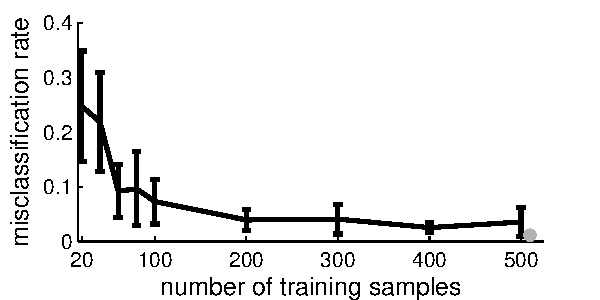
\includegraphics[width=1.0\linewidth]{../figs/hetero_easy_n10_MC5000_QAP_vs_n.pdf}
	\caption{Inexact graph matching can be used to approximate a consistent shuffled graph classifier.  Data in this simulation was sampled from the independent edge model described above.  For each number of training samples, we tested using 5000 test samples, and repeated 10 times.  The gray dot indicates Bayes optimal performance. (NOTE TO CEP: actually, i forgot to QAP the test data to each training class in this example.  i think it would converge much ``faster'' if i included that step. that is, faster in $s$, but now testing requires performing 2 QAPs, whereas before, it did not, so it might actually take longer.  we will see soon, as i'm running that now.)}
	\label{fig:1}
\end{figure}


% section simulated_experiment (end)


\section{Unlabeled Connectome Classification} % (fold)
\label{sub:connectome_classification}

Inspired by the simulated performance of our unlabeled graph classifier, we decided to try it on a real-world application.  A ``connectome'' is a graph in which vertices correspond to biological neural nodes, and edges correspond to connections between the nodes.  Diffusion Magnetic Resonance (MR) Imaging and related technologies are making the acquisition of MR connectomes routine \cite{Hagmann2010}.  49 subjects from the Baltimore Longitudinal Study on Aging comprise this data, with acquisition and connectome inference details as reported in \cite{Gray11}.  Each connectome yields a $70$ vertex simple graph (binary, symmetric, and hollow adjacency matrix).  Associated with each graph is class label based on the gender of the individual (24 males, 25 females).  Because the vertices are labeled, we can compare the results of having the labels and not having the labels.   Performance is evaluated with leave-one-out misclassification rate and reported in Table \ref{tab:connectome}. When using the vertex labels, a standard $k$nn achieves $20\%$ misclassification rate.  Chance performance (only using the estimated prior) on this data is $49\%$.  These two numbers provide bounds on performance.  When all graphs are passed through a shuffle channel, we first try to unshuffle the graphs using the above mentioned QAP algorithm.  Given the unshuffled graphs, performance changes to $45\%$, not particularly impressive.  The performance of the independent edge model based Bayes plugin classifier for unlabeled graphs is similarly unimpressive.  We therefore develop a hybrid approach in which the independent edge model is assumed, and parameters are estimated using the vertex labels.  Given these estimates, we can use the QAP algorithm to match each test graph to the two likelihood matrices, and then use the Bayes plugin classifier.  This approach yields a $31\%$ misclassification rate. In contrast, a ``standard'' graph invariant based approach, which computes the graph invariants from \cite{PCP10}, and plugs them into various machine learning algorithms (including the winner \cite{Crammer2008}), yields misclassification rates as low as $25\%$. 


% 
% \begin{itemize}
% 	\item \textbf{Graph Classifier} A Bayes plugin graph classifier as described in \cite{VP11a}; that is, using the labels.
% 	\item \textbf{1-QAP} Estimate the parameters using training data \emph{with} vertex labels.  Then, shuffle the test graph, \qap it to each $\mh{\PP}_y$ matrix.  The  estimated the class is $\mh{y}=\argmax_{y \in \mc{Y}}QAP(G,\mh{\PP}_y)$.   
% 	\item \textbf{48-QAP} Permuting the vertex labels, then implement \texttt{$1$NN$\circ$\qapa}.
% 	% \item \textbf{AVG-QAP}  Permuting the vertex labels, \qapa each of the 48 training graphs to the test graph.  Then, given those permuted adjacency matrices, compute the average, and then implement a standard $1$NN classifier.
% 	\item \textbf{1NN-GI} Use the graph invariant approach as described above. We provide the normalized graph invariants as inputs into a number of standard classifiers, including $k$NN, linear classifiers, support vector machines, random forests, and CW. On this data, the CW classifier performed best; we therefore only report its results.
% \end{itemize}
% 

\begin{table}[h!]
\caption{MR Connectome Leave-One-Out Misclassification Rates}
\begin{center}
\begin{tabular}{|r|r|r|r|r|}
\hline
\texttt{N/A-QAP} & \texttt{1-QAP} & \texttt{48-QAP} & \texttt{1NN-GI}\\
\hline
$20\%$ & $31\%$ & $45\%$  & $25\%$ \\
    \hline
\end{tabular}
\end{center}
\label{tab:connectome}
\end{table}%


\section{Discussion}

In this work, we have address both the theoretical and practical limitations of classifying graphs with and without including labels.  Specifically, we show that shuffling the vertex labels results in an irretrievable situation, with a possible degradation of classification performance, and a necessary degradation if the vertex labels contained class-conditional signal.  Moreover, although one cannot hope to recover the vertex labels, estimating them yields an asymptotically optimal classifier.  This suggest that efforts to estimate the vertex labels may yield useful classification results, outperforming ``standard'' graph-invariant based classifiers.  Via simulation we show that an approximate graph matching algorithm converges to the optimal performance with only about 500 training samples for a particular independent edge random graph model.   Finally, we demonstrate with connectome data that estimating the vertex labels can be useful, but that there remains room to grow to exceed misclassification performance of a carefully chosen graph invariant $\circ$ machine learning based approach on this data.   These connectome data, much like other collections of graphs, can also be equipped with both vertex and edge attributes.  As such, we hope to extend the results herein to consider the more general cases.








% use section* for acknowledgement
\ifCLASSOPTIONcompsoc
  % The Computer Society usually uses the plural form
  \section*{Acknowledgments}
\else
  % regular IEEE prefers the singular form
  \section*{Acknowledgment}
\fi


% Can use something like this to put references on a page
% by themselves when using endfloat and the captionsoff option.
\ifCLASSOPTIONcaptionsoff
  \newpage
\fi


\bibliography{/Users/jovo/Research/latex/library}
\bibliographystyle{IEEEtran}

\begin{IEEEbiography}{Joshua T. Vogelstein}
 is a spritely young man, engorphed in a novel post-buddhist metaphor.

\end{IEEEbiography}


% insert where needed to balance the two columns on the last page with
% biographies
%\newpage


\begin{IEEEbiography}{Carey E. Priebe}
Buddha in training.
\end{IEEEbiography}

% Can be used to pull up biographies so that the bottom of the last one
% is flush with the other column.
% \enlargethispage{-5in}

\end{document}



